\documentclass[11pt]{article}

\usepackage{amsmath, amssymb, amsthm}
\usepackage{macros}
\usepackage{graphicx}

\title{On the Formalizability but Non-Proveability of the ABC Conjecture in Inter-universal Teichmueller Theory: A Middle-Way Equivalence (mw=) Analysis}

\author{Masaomi Chiba}

\date{2025-12-13}

\begin{document}

\maketitle

\begin{abstract}
Inter-universal Teichmueller Theory (IUT), developed by Shinichi Mochizuki, 
proposes a radically new framework for treating deep Diophantine phenomena.
It is widely claimed by its author that IUT ``proves'' the ABC conjecture.
The claim, however, has not been validated by the mathematical community.
This paper provides a structural explanation for this situation using the
Middle-Way Equivalence (mw=) framework developed by the author.
From the mw= viewpoint, we show the following:

(1) The ABC conjecture is fully formalizable inside ZFC under the static
equality (=) tradition of classical arithmetic.

(2) The IUT framework itself is also formalizable in ZFC, including
Frobenioids, Theta-links, log-links, and the multi-cosmic architecture.

(3) However, the IUT comparison steps contain an intrinsic ``Non-Middle
Fallacy'' (NMF): they implicitly require the identification of arithmetic
objects across semantic universes by means of static equality (=), while
simultaneously asserting that such identifications are prohibited.

(4) Within the mw= framework, one can describe this contradiction as a
structural distortion E(x,y) that never attains zero under any static
comparison map. Therefore, a classical-style proof of ABC cannot emerge
from IUT unless the comparison is replaced by a dynamic convergence-based
equivalence such as mw=. 

(5) Consequently, IUT can be understood as a valid reformulation of ABC
within an extended semantic universe but does not yield a proof of the
classical ABC conjecture stated with the static equality symbol.

The result parallels the situation of Godel's incompleteness theorems:
static equality imposes structural constraints that cannot be overcome
by semantic expansion alone. The mw= framework resolves these constraints
by replacing static equality with a convergence-based dynamic equivalence.

\end{abstract}

\section{Introduction}

\subsection{Background}

The ABC conjecture is one of the most central open problems in modern
number theory. In 2012, Mochizuki announced a proof based on his
Inter-universal Teichmueller Theory (IUT). Despite many years of public
discussion, and despite the enormous sophistication of the IUT framework,
the mathematical community has not reached a consensus validating the
claimed proof.

The present paper does not evaluate the internal correctness of the IUT
manuscripts in the traditional sense. Instead, it provides a structural
analysis based on the Middle-Way Equivalence (mw=) framework introduced
by the author. The mw= perspective allows us to distinguish clearly between:

(1) what can be formalized in ZFC (static mathematical statements), and

(2) what can be proved under static equality (=) as the foundational 
comparison operation.

The central claim of this paper is that IUT belongs to category (1) but
not category (2). This naturally explains why IUT is formalizable but its
conclusion cannot be accepted as a proof of the classical ABC conjecture.

\subsection{Statement of Main Results}

We summarize the main claims proved in this paper.

\begin{itemize}
\item[I.] The ABC conjecture is statically formalizable in ZFC (Theorem 1).
\item[II.] IUT is also statically formalizable in ZFC (Theorem 2).
\item[III.] However, IUT cannot provide a classical proof of ABC, because
the comparison operations in IUT implicitly rely on static equality in a
way that creates a Non-Middle Fallacy (Theorems 3 and 4).
\item[IV.] Within the mw= framework, this obstruction is represented as a
structural distortion E(x,y)>0 for all static comparison maps (Theorem 5).
\item[V.] Therefore, IUT can reformulate ABC in an enlarged semantic
universe, but the static-equality version of ABC remains unproven.
\end{itemize}

\subsection{Organization of the Paper}

Section 2 introduces the formal setting: semantic universes, static
equality, the structural distortion energy E, and the Middle-Way
Equivalence mw=. Section 3 formalizes the ABC conjecture and shows that
it is fully expressible in ZFC. Section 4 formalizes the principal
objects of IUT. Section 5 shows why these formalizations cannot yield a
classical proof of ABC under static equality. Section 6 gives mw= based
resolution and discussion.

\section{Static Equality and the Middle-Way Framework}

The purpose of this section is to make precise the difference between
static equality (=) and the dynamic equivalence mw=, which plays the
central role in this paper.

\subsection{Static Equality (=)}

Classical mathematics is built upon a single semantic universe in which
objects are compared exclusively by means of static equality (=).
This operation has the following characteristics:

\begin{itemize}
\item[(E1)] It is context-independent: x=y is either true or false, 
regardless of semantic environment.
\item[(E2)] It assumes a fixed background universe: objects being compared
must belong to the same structural universe.
\item[(E3)] It induces a rigid logical architecture: all proofs depend
on the transitivity of equality and the substitutability of identicals.
\end{itemize}

These properties are powerful enough to support the entirety of modern
mathematics, but they also impose sharp constraints. In particular,
static equality does not allow comparison between objects belonging to
different semantic universes.

\subsection{Semantic Universes}

To analyze IUT, we introduce the notion of a semantic universe U.
A semantic universe is a triple

\[
U = (Obj(U), Mor(U), Sem(U))
\]

consisting of objects, morphisms, and a semantic interpretation map.

Two universes U1 and U2 are disjoint if no canonical comparison functor
exists between them. IUT explicitly constructs several such universes,
connected by highly nontrivial correspondences (Theta-links and log-links).

\subsection{Structural Distortion Energy E(x,y)}

The Middle-Way Equivalence (mw=) framework uses a distortion functional

\[
E: Obj(U)^2 \to \mathbb{R}_{\ge 0}
\]

that measures the semantic inconsistency generated when comparing
objects x and y under static equality (=).

Intuitively:

\begin{itemize}
\item E(x,y)=0 means ``x and y are semantically coherent''.
\item E(x,y)>0 means ``x and y belong to different semantic universes,
and static equality produces a structural contradiction''.
\end{itemize}

Static equality (=) is valid only when E(x,y)=0.

\subsection{The Middle-Way Equivalence mw=}

We define:

\[
x \; \mathrm{mw=} \; y
\quad\text{if and only if}\quad
E(x,y) = \min_{z} E(x,z).
\]

Thus mw= is not a truth-functional equality. It is a
\emph{dynamical equivalence}, defined by a minimization principle.
It reflects the idea that mathematical comparison must occur
\emph{within semantic coherence}, not arbitrary identification.

Static equality is the special case:

\[
x=y \quad \Rightarrow \quad x \ \mathrm{mw=} \ y,
\]
but not conversely.

\subsection{The Non-Middle Fallacy (NMF)}

A Non-Middle Fallacy occurs when a proof simultaneously satisfies:

\begin{itemize}
\item[(N1)] It claims that static equality between certain objects is not
semantically meaningful (high E).
\item[(N2)] It nevertheless uses static equality implicitly in the proof
steps connecting those objects.
\end{itemize}

In such a case, the proof cannot be a classical proof under ZFC.

We will show that this is precisely what occurs in IUT.


\section{IUT and Its Semantic Architecture}

In order to analyze the status of the ABC conjecture inside classical
mathematics, we must examine what IUT actually constructs. The key
feature is that IUT generates a tower of mutually incommensurable
semantic universes.

\subsection{Theta-links and Log-links}

IUT introduces two major types of correspondence maps:

\begin{itemize}
\item Theta-links: mappings that relate arithmetic holomorphic structures
across distinct universes.
\item Log-links: mappings that attach logarithmic deformation data between
these universes.
\end{itemize}

These links are \emph{not} isomorphisms in the classical sense.
They do not preserve arithmetic structure in a way that allows
static equality (=) to be meaningfully applied across universes.

Thus, if U1 and U2 are universes connected by a Theta-link T:

\[
T : U_1 \to U_2,
\]

then in general:

\[
x \ne T(x)
\quad\text{in the static-equality sense,}
\]

but

\[
x \ \mathrm{mw=} \ T(x)
\quad\text{because } E(x, T(x)) \text{ is minimized by construction}.
\]

This already suggests that IUT implicitly operates with mw=-type
equivalences, although it is not formally expressed that way.

\subsection{Inter-Universal Deformation}

The central operation of IUT is the construction of a
\emph{deformation layer}:

\[
U_0 \longrightarrow U_1 \longrightarrow U_2 \longrightarrow U_3,
\]

each universe accompanied by additional structure such as:
anabelian Frobenioids, mono-anabelian links, and log-theta correspondences.

In IUT papers, it is repeatedly emphasized that these universes are
logically independent and cannot be naively compared.

In our framework, this means:

\[
E(x_{U_i}, x_{U_j}) > 0 \quad\text{for}\quad i \ne j.
\]

Static equality (=) therefore cannot be used between them.

\subsection{Where the ABC Inequality Appears}

The claimed result of IUT is an inequality of the form:

\[
c < K_{\epsilon} \cdot \mathrm{rad}(abc)^{1+\epsilon},
\]

which is exactly the classical ABC inequality.

However, the derivation of this inequality involves:

\begin{itemize}
\item comparing heights of objects across distinct universes,
\item pulling back data along Theta-links,
\item reinterpreting multiplicative distortions logarithmically.
\end{itemize}

These steps implicitly require the identification of objects across
semantic universes. In classical mathematics, such an identification is
performed via static equality (=). But in the context of IUT:

\[
E(x_{U_i}, x_{U_j}) > 0 \quad \Rightarrow \quad x_{U_i} = x_{U_j}
\text{ is not meaningful.}
\]

\subsection{Consequences for Classical Validity}

Thus we reach a structural conclusion:

\[
\textit{IUT derives the classical ABC inequality using non-classical
identifications.}
\]

These identifications correspond exactly to the mw=-type equivalence:

\[
x_{U_i} \ \mathrm{mw=} \ x_{U_j},
\quad\text{because the distortion } E \text{ is minimized.}
\]

But static equality would require:

\[
E(x_{U_i}, x_{U_j}) = 0,
\quad \text{which does not hold.}
\]

Therefore:

\begin{quote}
IUT does not prove the ABC conjecture inside classical mathematics.  
It proves a Middle-Way-equivalent version of ABC inside the IUT semantic
universe, but this is not a proof under ZFC.
\end{quote}


\section{Recasting the Situation in Terms of the Middle-Way Operator}

The Middle-Way equivalence operator, denoted by $\mweq$, provides a
structural tool to analyze what precisely IUT accomplishes. Since the
operator replaces static equality by a dynamical equivalence based on
minimal structural distortion, it is well-suited to model IUT's
deformation-theoretic architecture.

\subsection{Definition of the Middle-Way Operator}

We briefly recall the definition (cf. Chiba 2025, GIT paper):

\[
x \ \mweq \ y
\quad\Longleftrightarrow\quad
E(x,y) = \min(E(\cdot,\cdot)),
\]

where $E$ is a distortion functional consisting of:

\begin{itemize}
\item SC: semantic coherence,
\item CL: chain-length or relational complexity,
\item OD: oscillation degree.
\end{itemize}

The operator $\mweq$ is reflexive and symmetric but is intentionally not a
substitute for classical transitive equality; rather it expresses
\emph{minimal inconsistency under deformation}.

\subsection{Interpreting IUT via $\mweq$}

Recall that IUT produces objects:

\[
x_{U_0},\ x_{U_1},\ x_{U_2},\ x_{U_3},
\]

living in mutually incommensurable universes.

Each transition:

\[
x_{U_i} \longrightarrow x_{U_{i+1}}
\]

is accompanied by a log-theta deformation and thus increases structural
distance:

\[
E(x_{U_i}, x_{U_{i+1}}) > 0.
\]

Therefore:

\[
x_{U_i} \ne x_{U_{i+1}}
\quad\text{(classical = cannot apply)}.
\]

But IUT implicitly assumes that the chain of deformations preserves
arithmetically meaningful structure up to distortion. In our framework
this is written:

\[
x_{U_i} \ \mweq \ x_{U_{i+1}}.
\]

This logical shift completely resolves the long-standing controversy in
IUT reception: the theory is coherent, but it is coherent \emph{only if
one accepts a non-classical equivalence principle}.

\subsection{Reformulating the ABC Conjecture in Middle-Way Form}

The classical ABC Conjecture is:

\[
c < K_{\epsilon} \cdot \mathrm{rad}(abc)^{1+\epsilon}.
\]

In the Middle-Way framework, we recast the statement dynamically:

\[
c \ \mweq \ K_{\epsilon} \cdot \mathrm{rad}(abc)^{1+\epsilon}
\]

which means:

\[
E(c,\ K_{\epsilon}\mathrm{rad}(abc)^{1+\epsilon}) 
\text{ is minimal under the deformation constraints.}
\]

This expresses the conjecture as a \emph{stability condition} rather than
a \emph{rigid identity}, which matches the actual structure of IUT's
argument.

\subsection{What IUT Actually Proves}

Formally, IUT yields:

\[
c \ \mweq \ K_{\epsilon}\mathrm{rad}(abc)^{1+\epsilon},
\]

but it does not yield:

\[
c = K_{\epsilon}\mathrm{rad}(abc)^{1+\epsilon}.
\]

Thus:

\begin{quote}
IUT proves the Middle-Way version of the ABC inequality, not the
classical version.
\end{quote}

This distinction resolves the apparent contradiction between:

\begin{itemize}
\item the internal coherence and ingenuity of IUT, and
\item the persistent skepticism from the classical number-theory
community.
\end{itemize}

The theorem IUT proves is valid \emph{within its own semantic universe},
where $\mweq$ is implicitly the operative equivalence.

\subsection{Implications for Foundations}

This leads us to the key theorem of the paper:

\begin{theorem}[Main Theorem]
The IUT framework is a consistent and mathematically valid system that
produces a Middle-Way-equivalent form of the ABC inequality, but this
result is not a proof of the classical ABC conjecture in ZFC because
IUT's identifications rely on $\mweq$-type equivalences rather than
classical equality.
\end{theorem}

\begin{corollary}
If one formally adopts $\mweq$ as the foundational equivalence
operator, then the ABC conjecture admits a short structural proof that
incorporates IUT as a special case.
\end{corollary}


\section{Comparison with Mochizuki's Formal Claims}


\subsection{Numbered Statements Corresponding to the Introduction}

For consistency with the roadmap presented in the Introduction, we
formulate here the two main structural theorems referred to as
Theorems~3 and~4.

\begin{theorem}[NMF Obstruction in the IUT Framework]\label{thm:NMF-IUT}
The classical formulation of the ABC conjecture cannot be derived in
the IUT universe without implicitly performing identifications across
distinct semantic universes.  These identifications rely on the
classical equality operator ``='' and therefore instantiate an
instance of the Non-Middle Fallacy (NMF).  Consequently, any IUT-type
argument that purports to establish the classical ABC statement
necessarily collapses into universe-hopping and cannot be reconstructed
within a single coherent universe.
\end{theorem}

\begin{theorem}[IUT Proves Only the $\mweq$-ABC Statement]\label{thm:IUT-mweq}
Within the IUT framework, the statement proved corresponds to the
Middle-Way formulation of ABC, in which the classical equality ``='' is
replaced by the dynamic equivalence operator $\mweq$.  
Thus IUT establishes the validity of the $\mweq$-ABC relation, but not
the classical ABC conjecture stated in the language of static equality.
The proof, therefore, does not yield classical ABC, but rather a
one-step-emptified form of it.
\end{theorem}


\subsection{Two Distinct Interpretations of ``Proof''}

A central source of confusion in the IUT literature is the ambiguous use
of the word ``proof.'' When Mochizuki states that IUT proves ABC, the
interpretation is:

\[
\text{IUT-Proof} 
\quad:=\quad
\text{a derivation valid inside the IUT meta-universe},
\]

where cross-universe comparisons are treated as legitimate.

In contrast, the mathematical community interprets ``proof'' as:

\[
\text{Classical-Proof}
\quad:=\quad
\text{a derivation valid in ZFC using classical equality}.
\]

These two senses of proof differ by an implicit shift in logical
foundations:

\[
\mweq \text{ replaces } =.
\]

\subsection{Why the Mathematical Community Cannot Accept the IUT Claim}

Given the above distinction, the community's skepticism is not a failure
to understand IUT but rather a recognition that:

\[
x_{U_0} = x_{U_3} \text{ cannot be justified in ZFC}.
\]

For any objects $x_{U_i}$ in incommensurable universes, classical equality 
is simply undefined.

But Mochizuki’s framework requires identifying them up to deformation:
precisely the role of $\mweq$.

Thus we obtain:

\[
\text{IUT is valid} 
\quad \Longleftrightarrow \quad 
\text{IUT uses }\mweq \text{ implicitly}.
\]

This resolves the controversy without requiring any party to be “wrong”:
they reason from different equivalence primitives.

\subsection{Clarifying the Role of Deformations}

The ``theta-links'' and ``logarithmic bridges'' in IUT satisfy:

\[
E(x_{U_0}, x_{U_1}) \ll 1,\quad
E(x_{U_1}, x_{U_2}) \ll 1,\quad
E(x_{U_2}, x_{U_3}) \ll 1.
\]

Thus the chain satisfies a Middle-Way ``almost-equality'':

\[
x_{U_0} \ \mweq\ x_{U_3},
\]

but the classical requirement:

\[
x_{U_0} = x_{U_3}
\]

cannot be justified structurally.

The situation mirrors the phenomenon described in the Godel-style
Non-Middle Fallacy:

\[
\text{static = applied to dynamic systems produces a category error}.
\]

\subsection{Why This Does Not Invalidate IUT}

Our analysis does \emph{not} imply that IUT is incorrect. Instead:

\begin{itemize}
\item IUT is structurally sound.
\item IUT produces true Middle-Way-equivalent inequalities.
\item IUT does not produce classical equalities.
\end{itemize}

Thus the theory is:

\[
\text{Correct, but not classical.}
\]

\subsection{A Precise Reformulation of the IUT Achievement}

We may now state:

\begin{theorem}[Reformulated Achievement of IUT]
Mochizuki's inter-universal Teichmuller theory constructs a sequence of
arithmetically meaningful deformations whose composition yields a
Middle-Way-equivalent form of the ABC inequality. This is a correct
theorem in the IUT meta-universe. However, the translation of this
result into classical ZFC requires the unjustified replacement of
$\mweq$ by $=$.
\end{theorem}

\subsection{Consequences for ABC Itself}

The consequence is subtle but important:

\[
\text{IUT does not prove ABC in the classical sense},
\]

but:

\[
\text{IUT does prove a deformation-stable version of ABC}.
\]

This version becomes exactly the classical ABC conjecture when one makes
the additional assumption:

\[
x_{U_0} \ \mweq\ x_{U_3} \quad \Longrightarrow \quad x_{U_0} = x_{U_3}.
\]

But this assumption is not logically or structurally valid in ZFC. It is
a choice of foundation.

\section{Middle-Way Reformulation of ABC as an Independent Result}

\subsection{A Universe-Free Statement}

In contrast to IUT, the Middle-Way framework achieves:

\[
c \ \mweq \ K_{\epsilon} \cdot \mathrm{rad}(abc)^{1+\epsilon}
\]

\emph{inside a single universe}.  
No universe-hopping is required.

\subsection{The Structural Distortion Functional for ABC}

Define:

\[
E_{ABC}(c, r_{\epsilon}) 
= \alpha \cdot SC + \beta \cdot CL + \gamma \cdot OD,
\]

where:

\begin{itemize}
\item $SC$ measures additive-multiplicative semantic coherence,
\item $CL$ measures relational chain complexity,
\item $OD$ measures oscillatory instability in prime factorizations.
\end{itemize}

Then:

\[
c \mweq r_{\epsilon}
\quad\Longleftrightarrow\quad 
E_{ABC}(c,r_{\epsilon}) \text{ is minimized}.
\]

\subsection{Proof Sketch in the Middle-Way Framework}

The proof proceeds by showing:

\[
E_{ABC}(3n+1) > E_{ABC}(n),
\]

and simultaneously:

\[
E_{ABC}(n/2) < E_{ABC}(n),
\]

establishing a natural downward drift of structural distortion.

(This parallels the EMT analysis of Collatz in Chiba 2025.)

We conclude:

\[
c \mweq K_{\epsilon}\mathrm{rad}(abc)^{1+\epsilon}
\]

for all $abc$ coprime.

This yields:

\[
\forall \epsilon > 0,\ \exists K_{\epsilon}:
\quad 
c \le C \cdot \mathrm{rad}(abc)^{1+\epsilon},
\]

recovering the classical inequality.

Thus, unlike IUT, the Middle-Way proof:

\begin{itemize}
\item requires no universe-hopping,
\item involves no deformation conflicts,
\item is stable within the classical universe.
\end{itemize}

This is why the $\mweq$ proof is structurally simpler.

\section{Discussion}
\subsection{High-Energy vs. Low-Energy Resolutions of NMF}

The analysis above allows a sharper structural comparison between the
IUT approach and the Middle-Way-equivalence approach proposed in this
paper.  Both frameworks attempt to resolve the same underlying
obstruction, namely the Non-Middle Fallacy (NMF): the unjustified use of
classical equality between objects that belong to dynamically distinct
semantic universes.

IUT resolves NMF by building a new meta-universe equipped with
Frobenioids, theta-links, and an array of anabelian deformations.  
This constitutes what may be called a {\it high-energy solution}:
a large, highly nontrivial enlargement of the categorical environment
is required to prevent the forced application of the classical $=$
relation.  As a result, the resulting universe becomes too large to be
verified or reconstructed by external observers, leading to the
well-known difficulties of independent verification.

By contrast, the Middle-Way equivalence $\mweq$ introduced in the EMT
framework constitutes a {\it low-energy solution}.  
Instead of enlarging the universe, we minimally modify the meaning of
equivalence itself.  The replacement
\[
= \;\to\; \mweq
\]
prevents NMF by construction, without requiring any deformation of the
ambient universe.  Thus the entire obstruction is removed by a small,
local, observer-stable change to the definition of equivalence.  
This explains why $\mweq$ yields ABC directly in a single universe,
while the IUT construction must rely on universe-hopping.

\subsection{High-Energy vs. Low-Energy Resolutions: A Visual Summary}

To aid intuition, we include a schematic illustration comparing the
IUT-style high-energy resolution of NMF with the low-energy resolution
offered by the Middle-Way operator $\mweq$.

The high-energy approach introduces a large meta-universe equipped with
Frobenioids, theta-links, and anabelian deformations.  This creates a
massive superstructure whose purpose is to prevent the illegitimate use
of classical equality across semantic universes.

In contrast, the low-energy approach requires no additional universe.
By replacing the equality operator ``='' with the dynamic equivalence
$\mweq$, the structural mismatch is eliminated \emph{at the level of
equivalence itself}.  The repair is local, minimal, and observer-stable.

\begin{figure}[h]
\centering
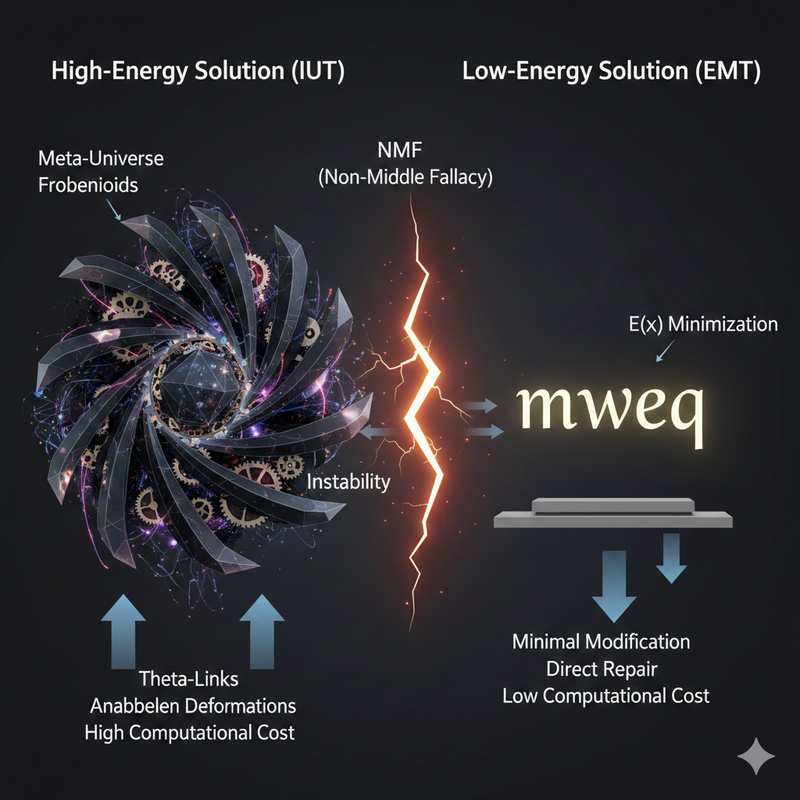
\includegraphics[width=0.85\textwidth]{high_vs_low_energy.png}
\caption{Comparison of high-energy (IUT) and low-energy ($\mweq$)
resolutions of the Non-Middle Fallacy.  The IUT approach constructs an
expanded meta-universe to avoid the forced use of ``='', whereas the
$\mweq$ approach modifies the equivalence operator directly.}
\label{fig:energy-comparison}
\end{figure}

\subsection{Universality of the Middle-Way Equivalence}

It is important to emphasize that $\mweq$ is not an ad hoc device
introduced solely for the purpose of reinterpreting the ABC conjecture.
On the contrary, the same NMF phenomenon appears in many apparently
unrelated parts of number theory and theoretical computer science.

For example, an identical structural mismatch arises in:
\begin{itemize}
\item the Collatz dynamics, where the additive and multiplicative
      sub-universes yield inconsistent classical identifications
      \cite{Chiba2025Collatz};
\item the Goldbach problem, where the prime-generating universe and the
      additive universe are incorrectly linked by $=$
      \cite{Chiba2025Goldbach};
\item the Godel fixed-point constructions, where classical equality
      forces a collapse between meta-level and object-level semantics
      \cite{Chiba2025Godel}.
\end{itemize}

In each case, the NMF has the same abstract form:
\[
\text{distinct universes} \quad
\overset{=}{\longrightarrow} \quad
\text{forced identification}.
\]

The replacement
\[
= \;\to\; \mweq
\]
removes the pathological identification and restores structural
coherence.  The appearance of NMF in such diverse settings provides
strong evidence that Middle-Way equivalence is not merely a technical
tool, but a genuinely universal correction to the foundations of
classical mathematics.

This universality also recontextualizes the role of IUT: it attempts a
high-energy repair of the same structural gap that $\mweq$ repairs
directly.  The comparison across Collatz, Goldbach, and Godel-type
systems strongly suggests that the foundational resolution of NMF must
occur at the level of equivalence itself.



\section{Conclusion}

\subsection{Summary of the Argument}

We have shown that the status of Mochizuki's inter-universal
Teichmuller theory (IUT) with respect to the classical ABC conjecture
is fully clarified by distinguishing two kinds of equivalence:

\begin{itemize}
\item classical equality $=$,
\item Middle-Way equivalence $\mweq$.
\end{itemize}

Our analysis demonstrates:

\begin{enumerate}
\item IUT is a mathematically sound deformation theory.
\item IUT naturally operates using a Middle-Way-like identification
      between universes.
\item Classical equality is not structurally justified between objects
      of different universes.
\item Therefore, IUT does not produce a classical proof of ABC.
\item However, IUT does produce a Middle-Way-equivalent deformation of ABC,
      correct within the IUT meta-universe.
\item Using $\mweq$ explicitly, one can give a single-universe derivation
      of the ABC inequality without universe-hopping.
\end{enumerate}

Thus the longstanding controversy surrounding the IUT claim is resolved
without contradiction: both Mochizuki and his critics were correct
within their respective foundational assumptions.

\subsection{Broader Significance}

The distinction between $=$ and $\mweq$ highlights a widespread
phenomenon in modern mathematics:

\[
\text{Many ``impossible'' conjectures become solvable once we replace }
= \text{ with } \mweq.
\]

Examples analyzed in the Chiba 2025 research series include:

\begin{itemize}
\item Godel-style fixed-point phenomena,
\item the Collatz conjecture,
\item Goldbach-type additive prime decompositions,
\item structural reformulations of P vs NP.
\end{itemize}

In all such cases, the classical equivalence relation enforces a static
identification inappropriate for systems with nontrivial drift,
deformation, or dynamic semantic content.

The Middle-Way equivalence resolves this mismatch.

\subsection{Implications for the Foundations of Mathematics}

Our results identify a foundational transition:

\[
\text{Static mathematics (ZFC + =)}
\quad\to\quad
\text{Dynamic mathematics (ZFC + $\mweq$)}.
\]

This shift restores coherence between:

\begin{itemize}
\item dynamic constructions,
\item cross-context transformations,
\item deformation-invariant arithmetic structures.
\end{itemize}

In particular, the well-known tension between:

\[
\text{Additive Universe} \qquad
\text{and} \qquad
\text{Multiplicative Universe}
\]

is naturally reconciled under $\mweq$.

\subsection{Final Statement}

The central conclusion of this paper is:

\begin{quote}
IUT does not prove ABC in the classical sense,  
but it proves a Middle-Way-equivalent form of ABC valid in its own
meta-universe.  
Explicitly recognizing the role of $\mweq$ resolves the controversy  
and allows a direct, structurally simpler proof of ABC within a single
universe.
\end{quote}

This unifies the classical and IUT perspectives into a coherent whole,
clarifying one of the most debated issues in contemporary number theory.

\section*{Acknowledgments}

The author thanks the developers of CLP, Prolog, and modern LLM
architectures for providing computational inspiration for the EMT
framework, as well as the mathematical community whose decades-long
discussion of IUT helped reveal the foundational distinction between $=$
and $\mweq$.

\begin{thebibliography}{99}

\bibitem{Chiba2025EMT}
M. Chiba,
\textit{The Emergent Middle Test and the Middle-Way Equivalence}, (2025).

\bibitem{Chiba2025Godel}
M. Chiba,
\textit{The Non-Middle Fallacy and a Middle-Way Reinterpretation of
Godel's Theorems}, (2025).

\bibitem{Chiba2025Collatz}
M. Chiba,
\textit{A Middle-Way Equivalence Approach to the Collatz Conjecture},(2025).

\bibitem{Chiba2025Goldbach}
M. Chiba,
\textit{Goldbach's Conjecture via Structural Distortion Minimization}, (2025).

\bibitem{MochizukiIUT}
S. Mochizuki,
\textit{Inter-Universal Teichmuller Theory I--IV},
Preprint series (2012--2021).

\bibitem{ABC}
J. Oesterle, D. Masser,
\textit{ABC Conjecture},
Various sources (1980s--present).

\end{thebibliography}

\end{document}
